\documentclass[11pt]{article}

\usepackage[utf8]{inputenc}
\usepackage[T1]{fontenc}
\usepackage[english]{babel}
\usepackage[a4paper,margin=1.08in]{geometry}
\IfFileExists{newtxtext.sty}{\usepackage{newtxtext,newtxmath}}{\usepackage{lmodern}}
\usepackage{microtype}
\usepackage{amsmath,amssymb,amsthm,mathtools}
\usepackage{booktabs,graphicx,xcolor}
\usepackage[font=small,labelfont=bf]{caption}
\usepackage[numbers,sort&compress]{natbib}
\usepackage[colorlinks=true,linkcolor=blue!45!black,citecolor=blue!45!black,urlcolor=blue!45!black]{hyperref}

\newtheorem{definition}{Definition}[section]
\newtheorem{proposition}[definition]{Proposition}
\newtheorem{lemma}[definition]{Lemma}
\newtheorem{remark}[definition]{Remark}
\newtheorem{assumption}[definition]{Assumption}
\newtheorem{example}[definition]{Example}

\newcommand{\A}{\mathcal A}
\newcommand{\V}{\mathcal V}
\newcommand{\X}{\mathcal X}
\newcommand{\E}{\mathbb E}
\newcommand{\N}{\mathbb N}
\newcommand{\R}{\mathbb R}
\newcommand{\1}{\mathbf 1}
\newcommand{\KL}{D_{\mathrm{KL}}}
\newcommand{\softmax}{\operatorname{softmax}}
\newcommand{\PPL}{\operatorname{PPL}}
\newcommand{\code}[1]{\texttt{#1}}

\title{\bfseries Empirical Textual Diversity and Predictive Risk\\in Character-Level Autoregressive Models}
\author{Nicolás Meléndez\\Universidad de los Andes, Bogotá\\\texttt{nicolasmelendez30@gmail.com}}
\date{2026}

\begin{document}
\maketitle

\begin{abstract}
We study whether corpora with nearly equal character budgets but different
empirical diversity induce systematic differences in the predictive risk of
small autoregressive models. The statistical objects implemented by the
software are specified explicitly: a finite sample space of strings, empirical
measures on overlapping context windows, conditional probability kernels
defined by causal decoders, and a finite-sample optimization problem. The
experiment consists of one Transformer and one RMSNorm--RoPE--SwiGLU variant,
each trained once on a homogeneous corpus and on a mixture of authors. The
mixture has larger block entropy, distinct-$4$ ratio, and gzip byte ratio. Its
test loss is nevertheless larger for both architectures, whereas its empirical
test--train difference is smaller. These four fits do not identify a causal
effect of diversity: character distribution, domain, vocabulary, and parameter
count vary simultaneously, and only one initialization was observed. We
therefore treat the result as a computational description rather than a
population estimate. A unigram-adjusted contextual gain and a replicated
factorial design are specified for subsequent experiments.
\end{abstract}

\section{Problem statement}

Let $\A$ be a finite alphabet and let
$s=(s_0,\ldots,s_{N-1})\in\A^N$ be an observed string. No independence or
stationarity assumption is imposed on its coordinates. Empirical scaling laws
relate loss to parameter count, data, and computation
\cite{kaplan-2020-scaling,hoffmann-2022-chinchilla}; they do not imply that two
strings of the same length define statistically equivalent learning problems.
Chang et al. introduce quality corrections that replace raw token count by an
effective size \cite{chang-etal-2024-scaling}. The present experiment is not a
replication of that fit: it estimates no scaling coefficient, constructs no
scaling curve, and uses no teacher model.

For two strings $s^{(0)}$ and $s^{(1)}$ of approximately equal length, two
neural families, and a fixed optimization budget, we compare
\begin{align}
 L_j&=\widehat R_{\mathrm{te}}(\widehat w;s^{(j)}),\label{eq:test-risk}\\
 \Gamma_j&=\widehat R_{\mathrm{te}}(\widehat w;s^{(j)})-
 \widehat R_{\mathrm{tr}}(\widehat w;s^{(j)}),\quad j\in\{0,1\}.
 \label{eq:gap}
\end{align}
$L_j$ is absolute predictive loss on a held-out segment of the same corpus.
$\Gamma_j$ compares two empirical measures supported on different windows. It
is not itself a population generalization bound. Neither quantity identifies a
causal effect of diversity without further design assumptions.

\section{Measure-theoretic foundations}
\label{sec:measure}

This section fixes the probabilistic language used below. The material is
standard; proofs are included when they clarify a construction used by the
software. General versions can be found in
\cite{petersen-zech-2026-mathematical}.

\subsection{Measurable spaces and probability measures}

\begin{definition}[$\sigma$-algebra]
Let $\Omega$ be a set. A collection $\mathcal F\subseteq2^\Omega$ is a
$\sigma$-algebra if $\Omega\in\mathcal F$, if it is closed under complements,
and if it is closed under countable unions. The pair $(\Omega,\mathcal F)$ is a
measurable space.
\end{definition}

On a finite set $S$ we use the power set $2^S$. On $\R^d$ we use the Borel
$\sigma$-algebra $\mathcal B(\R^d)$ generated by the Euclidean open sets.

\begin{definition}[Measure]
A measure on $(\Omega,\mathcal F)$ is a function
$\mu:\mathcal F\to[0,\infty]$ such that $\mu(\varnothing)=0$ and
\[
 \mu\left(\bigcup_{n=1}^{\infty}A_n\right)
 =\sum_{n=1}^{\infty}\mu(A_n)
\]
for every sequence of pairwise disjoint $A_n\in\mathcal F$. It is a
probability measure if $\mu(\Omega)=1$. A probability space is a triple
$(\Omega,\mathcal F,\mathbb P)$.
\end{definition}

For $\omega\in\Omega$, the Dirac measure is
$\delta_\omega(A)=\1\{\omega\in A\}$. Hence the empirical measure of
$\omega_1,\ldots,\omega_n$ is $n^{-1}\sum_i\delta_{\omega_i}$. This formula,
rather than informal language about a ``dataset distribution'', defines every
empirical risk in this paper.

\begin{definition}[Random variable and law]
Let $(\Omega,\mathcal F)$ and $(S,\mathcal S)$ be measurable spaces. A map
$X:\Omega\to S$ is measurable if $X^{-1}(A)\in\mathcal F$ for every
$A\in\mathcal S$. If $X$ is defined on a probability space, it is an
$S$-valued random variable. Its law is the pushforward measure
\[
 \mathbb P_X=\mathbb P\circ X^{-1},
 \qquad \mathbb P_X(A)=\mathbb P(X\in A).
\]
\end{definition}

If $S$ is finite, a probability law is a vector $(p_s)_{s\in S}$ with
$p_s\ge0$ and $\sum_sp_s=1$. Integration then reduces to summation:
\[
 \E[g(X)]=\int_\Omega g(X(\omega))\,d\mathbb P(\omega)
 =\sum_{s\in S}g(s)p_s.
\]

\subsection{Conditioning}

\begin{definition}[Conditional expectation]
Let $Z$ be integrable and $\mathcal G\subseteq\mathcal F$. A conditional
expectation $\E[Z\mid\mathcal G]$ is a $\mathcal G$-measurable integrable
random variable satisfying
\[
 \int_G\E[Z\mid\mathcal G]\,d\mathbb P
 =\int_G Z\,d\mathbb P
 \quad\text{for every }G\in\mathcal G.
\]
It is unique up to almost-sure equality.
\end{definition}

If $X,Y$ are finite-valued with joint mass $p(x,y)$ and $p_X(x)>0$, then
\[
 p(y\mid x)=\frac{p(x,y)}{p_X(x)},
 \qquad
 \E[g(Y)\mid X=x]=\sum_y g(y)p(y\mid x).
\]
The conditional mass $p(\cdot\mid x)$ is the object approximated by a
next-token model.

\begin{proposition}[Tower property; standard]
If $Z$ is integrable and $\mathcal H\subseteq\mathcal G\subseteq\mathcal F$,
then
\[
 \E[\E[Z\mid\mathcal G]\mid\mathcal H]
 =\E[Z\mid\mathcal H]
 \quad\text{almost surely}.
\]
In particular, $\E[\E[Z\mid\mathcal G]]=\E[Z]$.
\end{proposition}

\subsection{Stochastic processes and probability kernels}

\begin{definition}[Stochastic process and filtration]
For an index set $T$ and a measurable state space $S$, a stochastic process is
a family $(X_t)_{t\in T}$ of $S$-valued random variables on one probability
space. For $T=\N_0$, its natural filtration is
\[
 \mathcal F_t^X=\sigma(X_0,\ldots,X_t),
\]
the information generated up to time $t$.
\end{definition}

\begin{definition}[Markov property]
A discrete process $(X_t)$ is a first-order Markov process if, for every $t$
and every state $a$,
\[
 \mathbb P(X_{t+1}=a\mid\mathcal F_t^X)
 =\mathbb P(X_{t+1}=a\mid X_t)
 \quad\text{almost surely}.
\]
\end{definition}

An autoregressive language model need not be first-order Markov: its kernel may
depend on the whole available context. The bigram model is first-order Markov.
A causal decoder instead satisfies an adaptedness requirement: its logits at
time $t$ may depend on $\mathcal F_t^X$ but not on future tokens.

\begin{definition}[Probability kernel]
For measurable spaces $(S,\mathcal S)$ and $(T,\mathcal T)$, a probability
kernel $K$ from $S$ to $T$ satisfies: (i) $K(s,\cdot)$ is a probability measure
for each $s$; and (ii) $s\mapsto K(s,A)$ is measurable for every
$A\in\mathcal T$.
\end{definition}

On finite alphabets measurability is automatic. The chain rule for a joint mass
function is a product of successive kernels; this is the measure-theoretic
content of autoregressive factorization.

\section{Statistical learning from first principles}
\label{sec:learning}

Let $(\mathcal U,\mathcal U_0)$ be an input space,
$(\mathcal Y,\mathcal Y_0)$ an output space, and $\mathcal O$ an action space.

\begin{definition}[Hypothesis, loss, and risk]
A hypothesis is a measurable map $h:\mathcal U\to\mathcal O$. A hypothesis
class $\mathcal H$ is a set of hypotheses. Given a measurable loss
$\ell:\mathcal O\times\mathcal Y\to[0,\infty]$ and a data law $P$ on
$\mathcal U\times\mathcal Y$, the population risk is
\[
 R_P(h)=\int\ell(h(u),y)\,dP(u,y).
\]
\end{definition}

\begin{definition}[Bayes risk and approximation error]
The Bayes and class-restricted risks are
\[
 R_P^*=\inf_{h\text{ measurable}}R_P(h),
 \qquad R_{P,\mathcal H}^*=\inf_{h\in\mathcal H}R_P(h).
\]
The quantity $R_{P,\mathcal H}^*-R_P^*\ge0$ is the approximation error of
$\mathcal H$ under $P$ and $\ell$.
\end{definition}

For observations $Z_i=(U_i,Y_i)$, define
\[
 \widehat P_n=\frac1n\sum_{i=1}^n\delta_{Z_i},
 \qquad
 \widehat R_n(h)=\int\ell(h(u),y)\,d\widehat P_n
 =\frac1n\sum_{i=1}^n\ell(h(U_i),Y_i).
\]

\begin{definition}[Learning algorithm]
A learning algorithm is a measurable map
$\mathfrak A:(\mathcal U\times\mathcal Y)^n\to\mathcal H$. Its output on
$S=(Z_1,\ldots,Z_n)$ is $\widehat h_S=\mathfrak A(S)$. An empirical risk
minimizer belongs to
$\operatorname*{argmin}_{h\in\mathcal H}\widehat R_n(h)$, when this set is
nonempty.
\end{definition}

The trained network is not known to be an exact empirical risk minimizer. It is
the output of a finite randomized algorithm; parameter initialization and
minibatch indices are part of that algorithm's randomness.

\begin{proposition}[Excess-risk decomposition; algebraic]
Suppose $h_{\mathcal H}^*$ minimizes $R_P$ over $\mathcal H$. For every
$\widehat h\in\mathcal H$,
\begin{align*}
 R_P(\widehat h)-R_P^*
 &=\underbrace{R_{P,\mathcal H}^*-R_P^*}_{\text{approximation}}\\
 &+\underbrace{R_P(\widehat h)-\widehat R_n(\widehat h)
 +\widehat R_n(h_{\mathcal H}^*)-R_P(h_{\mathcal H}^*)}_{
 \text{estimation/generalization}}\\
 &+\underbrace{\widehat R_n(\widehat h)-
 \widehat R_n(h_{\mathcal H}^*)}_{\text{empirical optimization}}.
\end{align*}
\end{proposition}

\begin{proof}
Add and subtract $\widehat R_n(\widehat h)$,
$\widehat R_n(h_{\mathcal H}^*)$, and $R_P(h_{\mathcal H}^*)$; then group
terms. The identity uses no probabilistic assumption.
\end{proof}

The decomposition explains why a cross-corpus loss difference cannot be
assigned to one mechanism. Changing a corpus may alter Bayes risk,
approximation error, finite-sample deviation, and the optimization landscape.

If $Z_1,\ldots,Z_n$ are iid from $P$ and $h$ is fixed independently of the
sample, then $\E[\widehat R_n(h)]=R_P(h)$. If also
$0\le\ell\le M$, Hoeffding's inequality yields
\[
 \mathbb P(|\widehat R_n(h)-R_P(h)|\ge\varepsilon)
 \le2\exp(-2n\varepsilon^2/M^2).
\]
For a data-dependent $\widehat h$, a pointwise bound is insufficient. One needs
uniform complexity control, stability, PAC-Bayes analysis, or another learning
theorem. None applies automatically to overlapping text windows, so no
population generalization bound is claimed here.

\section{Neural networks as parametric maps}
\label{sec:networks}

\subsection{Classical feedforward networks}

\begin{definition}[Affine layer]
For $m,n\in\N$, an affine layer is
$A_{W,b}:\R^n\to\R^m$, $A_{W,b}(x)=Wx+b$, where
$W\in\R^{m\times n}$ and $b\in\R^m$. It has $mn+m$ scalar parameters.
\end{definition}

An activation is a measurable scalar map extended coordinatewise. The models
use
\[
 \operatorname{GELU}(x)=x\Phi(x),
 \qquad
 \operatorname{SiLU}(x)=\frac{x}{1+e^{-x}},
\]
where $\Phi$ is the standard normal distribution function
\cite{hendrycks-2016-gelu,elfwing-2018-sigmoid}.

\begin{definition}[Feedforward neural network]
Let $d_0,\ldots,d_L\in\N$. A depth-$L$ feedforward network with activation
$\rho$ is the parametrized family $\Phi_\theta:\R^{d_0}\to\R^{d_L}$ given by
\begin{align*}
 h_0&=x,\\
 h_\ell&=\rho(W_\ell h_{\ell-1}+b_\ell),&&1\le\ell<L,\\
 \Phi_\theta(x)&=W_Lh_{L-1}+b_L,
\end{align*}
where $\theta$ concatenates all matrices and biases. Its hypothesis class is
$\{\Phi_\theta:\theta\in\Theta\}$.
\end{definition}

Modern architectures extend this base definition by composing differentiable
modules in a directed acyclic computation graph. Embedding lookup,
normalization, residual addition, attention, and multiplicative gating are such
modules. The Transformer is a neural network in this compositional sense.

\subsection{Embeddings and tensor-valued layers}

An embedding table is $E\in\R^{K\times d}$ with lookup $i\mapsto E_{i,:}$.
Equivalently, $E_{i,:}=e_i^\top E$ for a one-hot vector $e_i\in\R^K$.
Embedding lookup is therefore linear after the canonical inclusion of a token
into Euclidean space.

A sequence model acts on $H\in\R^{B\times d}$. Positionwise linear maps have
the form $H\mapsto HW$; normalization and activations act rowwise; attention
couples rows. Every finite tensor can be vectorized, so the architecture remains
a finite-dimensional parametrized map.

\subsection{Differentiation and backpropagation}

\begin{proposition}[Chain rule for a computation graph; standard]
Let $F=f_L\circ\cdots\circ f_1$, with differentiable
$f_j:\R^{d_{j-1}}\to\R^{d_j}$. If $h_j=f_j(h_{j-1})$, then
\[
 DF(x)=Df_L(h_{L-1})\cdots Df_1(x).
\]
For a scalar objective, reverse-mode differentiation evaluates the associated
transpose-Jacobian products from $L$ to $1$ and returns the gradient, up to
floating-point arithmetic.
\end{proposition}

\begin{proof}
The formula is the multivariate chain rule applied inductively. Associativity
permits the Jacobian product to be evaluated in reverse order without forming
each full Jacobian.
\end{proof}

Backpropagation is thus an efficient chain-rule algorithm, not an optimizer.
The resulting gradient is passed to SGD, AdamW, or another optimizer
\cite{rumelhart-1986-learning}.

Three questions must remain separate. \emph{Representation} asks which maps a
fixed architecture realizes exactly. \emph{Approximation} asks how closely a
growing architecture family approaches a target. \emph{Optimization} asks
whether an algorithm reaches a good parameter. Universal approximation, when
available, answers only the second question; it implies neither learnability
from finite data nor convergence of AdamW. No universal-approximation claim is
used in this experiment.

\section{Discrete representation and sample construction}

\subsection{Character tokenization}

\begin{definition}[Corpus-dependent tokenizer]
For a string $s$, define
\[
 \V(s)=\{a\in\A:\text{there exists }i\text{ such that }s_i=a\}.
\]
A character tokenizer is a bijection
\[
 \tau_s:\V(s)\longrightarrow\{0,\ldots,|\V(s)|-1\},
\]
extended coordinatewise to $\V(s)^n$ for every $n\in\N$. The implementation
orders $\V(s)$ lexicographically and stores both $\tau_s$ and $\tau_s^{-1}$.
\end{definition}

The transformation preserves length exactly. Since $\V(s)$ is constructed
from the complete string, including its test segment, no out-of-vocabulary
event can occur. This is a limited transductive use of test information: token
frequencies and order remain hidden, but the support is known before fitting.
A stricter protocol would construct a common vocabulary from training data and
include an unknown symbol.

Corpus-specific vocabularies also alter model capacity. If
$|\V(s^{(0)})|\ne|\V(s^{(1)})|$, the input embedding and output projection have
different dimensions. Losses are therefore reported in nats per character,
and parameter counts must be reported alongside them.

\subsection{Overlapping windows}

Fix a context length $B\in\N$. For $x_i=\tau_s(s_i)$ define
\begin{align}
 W_B(s)_i&=(X_i,Y_i),\qquad 0\le i<N-B,\\
 X_i&=(x_i,\ldots,x_{i+B-1}),\\
 Y_i&=(x_{i+1},\ldots,x_{i+B}).
\end{align}
The string is first divided into contiguous train, validation, and test
intervals with proportions $0.8$, $0.1$, and $0.1$. Windows are then formed
inside each interval, so no example crosses a split boundary.

\begin{proposition}[Deterministic overlap; project-specific]
For every admissible $i$, the input windows $X_i$ and $X_{i+1}$ share exactly
$B-1$ token positions. Consequently, the collection
$\{W_B(s)_i\}_{i=0}^{N-B-1}$ cannot be an iid sample unless the word ``sample''
refers only to randomized index selection from the finite collection.
\end{proposition}

\begin{proof}
The suffix $(x_{i+1},\ldots,x_{i+B-1})$ of $X_i$ is the prefix of
$X_{i+1}$ of the same length. The equality is deterministic and is independent
of any probabilistic law assigned to the original string.
\end{proof}

The reported standard deviations across randomly selected evaluation batches
therefore describe Monte Carlo variation of the implemented estimator. Without
a dependence model---for example, stationarity plus a suitable mixing
condition---the usual iid standard-error interpretation is unavailable.

\section{Probability model}

Let $K=|\V(s)|$ and
$\Delta_{K-1}=\{p\in[0,1]^K:\sum_{j=0}^{K-1}p_j=1\}$. For a fixed architecture,
$w\in\Theta\subset\R^p$ parametrizes a map
\[
 f_w:\{0,\ldots,K-1\}^{\le B}\longrightarrow\R^{B\times K}.
\]
The domain carries its power $\sigma$-algebra and the codomain its Borel
$\sigma$-algebra. Every such map is measurable because the domain is finite.

\begin{definition}[Autoregressive probability kernel]
For a context $x_{\le t}$, define
\begin{align}
 Q_w(j\mid x_{\le t})
   &=\softmax(f_w(x_{\le t})_{t,:})_j,\\
 \softmax(z)_j&=\frac{e^{z_j}}{\sum_{r=0}^{K-1}e^{z_r}}.
\end{align}
For fixed $x_{\le t}$, $Q_w(\cdot\mid x_{\le t})\in\Delta_{K-1}$.
\end{definition}

Given an initial distribution $\mu$ on $\V$, the finite-horizon law is
\begin{equation}
 Q_w^{(T)}(x_0,\ldots,x_{T-1})
 =\mu(x_0)\prod_{t=0}^{T-2}Q_w(x_{t+1}\mid x_{\le t}).
 \label{eq:factorization}
\end{equation}
Because the state space is finite, consistency of these kernels gives an
infinite-sequence law by the Ionescu--Tulcea construction. The implementation
only requires the finite-dimensional distributions in
\eqref{eq:factorization}.

Generation temperature $T_0>0$ replaces $z$ by $z/T_0$. Top-$k$ filtering
restricts the support to the indices of the $k$ largest logits and renormalizes
the resulting mass. Both operations modify the generative kernel; neither
appears in the training objective.

\section{Loss and risk}

\subsection{Logarithmic score}

For $z\in\R^K$ and $y\in\{0,\ldots,K-1\}$, set
\[
 \ell(z,y)=-\log\softmax(z)_y,
 \qquad
 L_B(w;X,Y)=\frac1B\sum_{t=0}^{B-1}\ell(f_w(X)_{t,:},Y_t).
\]
The derivative with respect to $z$ is
\[
 \nabla_z\ell(z,y)=\softmax(z)-e_y.
\]
Thus backpropagation begins with the difference between the predicted
probability vector and the one-hot observation.

\begin{proposition}[Conditional cross-entropy decomposition; standard]
Let $P$ be a probability measure on $\mathcal C\times\V$, where $\mathcal C$
is a finite context space, and let $q(\cdot\mid c)$ be strictly positive.
Then
\[
 \E_P[-\log q(Y\mid C)]
 =H_P(Y\mid C)+
 \E_{P_C}\!\left[\KL(P(\cdot\mid C)\|q(\cdot\mid C))\right].
\]
\end{proposition}

\begin{proof}
Condition on $C=c$, add and subtract $\log P(Y\mid c)$, and sum over
$c$ with respect to $P_C$. The first term is conditional entropy and the
second is the conditional Kullback--Leibler divergence.
\end{proof}

This identity is essential for interpreting cross-corpus loss. A larger test
loss can reflect larger irreducible conditional entropy, larger approximation
error, larger optimization error, or any combination of them. Raw loss does
not isolate model quality from task difficulty.

\subsection{Population and empirical measures}

Let $\mathsf P$ be a probability measure on
$\X=\V^B\times\V^B$. Its population risk is
\[
 R_{\mathsf P}(w)=\int_{\X}L_B(w;x,y)\,d\mathsf P(x,y).
\]
For a finite set of valid indices $I$, define the window empirical measure
\[
 \widehat{\mathsf P}_I=\frac1{|I|}\sum_{i\in I}\delta_{W_B(s)_i},
 \qquad
 \widehat R_I(w)=\int L_B(w;x,y)\,d\widehat{\mathsf P}_I(x,y).
\]
This definition is valid without an iid assumption. Such an assumption becomes
necessary only when $\widehat R_I$ is used to infer properties of an external
population law.

\subsection{Unigram adjustment}

To separate part of the marginal difficulty, the current evaluator fits on the
training split the add-$\alpha$ unigram model
\[
 \widehat q_\alpha(a)=\frac{n_{\rm tr}(a)+\alpha}
 {N_{\rm tr}+\alpha K},\qquad \alpha=1,
\]
and computes
\begin{align}
 L_{\rm uni}&=-\frac1{N_{\rm te}}
 \sum_{t\in I_{\rm te}}\log\widehat q_\alpha(x_t),\\
 G_{\rm ctx}&=L_{\rm uni}-\widehat R_{\rm te}(\widehat w),\\
 G_{\rm rel}&=G_{\rm ctx}/L_{\rm uni}.
\end{align}
$G_{\rm ctx}$ measures predictive gain over corpus-specific marginal
frequencies. It does not remove domain shift or identify a causal effect. Bits
per character and perplexity are
\[
 \operatorname{bpc}=\widehat R_{\rm te}/\log 2,
 \qquad \PPL=\exp(\widehat R_{\rm te}).
\]
They are monotone transformations of the same loss and must not be treated as
independent evidence.

\section{Model classes}

\subsection{Bigram kernel}

The reference model has $A\in\R^{K\times K}$ and
\[
 Q_A(x_{t+1}=j\mid x_{\le t})=\softmax(A_{x_t,:})_j.
\]
It is a homogeneous first-order Markov kernel. Its implementation as an
embedding table is exactly this parameterization, not an approximation to it.

\begin{proposition}[Closed-form bigram maximum likelihood; standard]
Let $n_{ij}$ be the number of observed transitions $i\to j$ and
$n_i=\sum_jn_{ij}$. Among all row-stochastic matrices $P$, every maximum of
\[
 \sum_{i,j}n_{ij}\log P_{ij}
\]
satisfies $P_{ij}=n_{ij}/n_i$ whenever $n_i>0$. Rows with $n_i=0$ are not
identified by the likelihood.
\end{proposition}

\begin{proof}
The objective separates by rows. For a fixed $i$ with $n_i>0$, divide by
$n_i$ and write $\widehat p_{ij}=n_{ij}/n_i$. Then
\[
 -\sum_j\widehat p_{ij}\log P_{ij}
 =H(\widehat p_i)+\KL(\widehat p_i\|P_i),
\]
which is minimized exactly at $P_i=\widehat p_i$ on the observed support.
\end{proof}

The trainable logit matrix is redundant: adding a constant to every entry of a
row leaves its softmax unchanged. This non-identifiability is benign for the
induced transition kernel but means the parameter minimizer is never unique
without an additional convention or penalty.

\subsection{Causal Transformer}

Each symbol is represented by $E(x_t)+P_t\in\R^d$. A pre-normalized block is
\begin{align*}
 H'&=H+\operatorname{MHA}(\operatorname{LN}(H)),\\
 H^+&=H'+\operatorname{FFN}(\operatorname{LN}(H')).
\end{align*}
For one head, set $Q=HW_Q$, $K'=HW_K$, and $V=HW_V$. Then
\begin{align}
 \operatorname{Attn}(H)&=\softmax_{\rm row}
 \left(\frac{QK'^{\top}}{\sqrt{d_h}}+M\right)V,\\
 M_{ts}&=\begin{cases}0,&s\le t,\\-\infty,&s>t.\end{cases}
\end{align}
The output at position $t$ is therefore a function only of $x_{\le t}$. The
repository tests this property by perturbing future tokens and checking exact
agreement of earlier logits. The feedforward sublayer is
$W_2\operatorname{GELU}(W_1h+b_1)+b_2$; a final affine map produces $K$
logits \cite{vaswani-2017-attention}.

For finite logits, each unmasked attention row is a probability vector. Hence
the pre-projection head output at position $t$ is a convex combination of
$v_0,\ldots,v_t$. This does not make the complete block a convex map: queries,
keys, values, softmax weights, residual paths, and the feedforward network all
depend nonlinearly on the input and parameters.

\begin{proposition}[Causal invariance; architecture-specific]
Let $F_w$ be a stack of the implemented masked attention blocks with
positionwise normalization, positionwise feedforward maps, and residual
connections. If two token sequences $x,x'$ agree through position $t$, then
their logits agree through position $t$:
\[
 x_{0:t}=x'_{0:t}
 \quad\Longrightarrow\quad
 F_w(x)_{0:t,:}=F_w(x')_{0:t,:}.
\]
\end{proposition}

\begin{proof}
Token and positional embeddings agree through $t$. Assume the hidden states
entering a block agree through $t$. Positionwise maps preserve this agreement.
At a position $r\le t$, the mask restricts attention to indices $s\le r$, on
which the hidden states agree; therefore queries, keys, values, weights, and
attention outputs agree. Residual addition preserves equality. Induction over
the two sublayers and then over blocks proves the claim; the final rowwise
normalization and output projection preserve it.
\end{proof}

\subsection{RMSNorm--RoPE--SwiGLU variant}

The second model preserves the residual causal decoder and changes three local
operators \cite{touvron-2023-llama}. First,
\[
 \operatorname{RMSNorm}(h)=g\odot
 \frac{h}{\sqrt{d^{-1}\|h\|_2^2+\varepsilon}}.
\]
Second, RoPE applies the planar rotation $R(t\theta_i)$ to each coordinate pair,
where $\theta_i=10000^{-2i/d_h}$ \cite{su-2021-roformer}. Since
\[
 R(t\theta)^{\top}R(s\theta)=R((s-t)\theta),
\]
the inner product between a rotated query and key depends on their relative
position. Third,
\[
 \operatorname{SwiGLU}(h)=W_d
 \bigl(\operatorname{SiLU}(W_gh)\odot W_uh\bigr).
\]
The term ``LLaMA-style'' refers only to these architectural choices; it does not
claim equivalence in scale, training regime, tokenizer, or every implementation
detail.

\section{Optimization theory}
\label{sec:optimization}

\subsection{First-order geometry}

Let $F:\R^p\to\R$ be differentiable. The gradient is characterized by
\[
 F(w+h)=F(w)+\langle\nabla F(w),h\rangle+o(\|h\|).
\]
Under the Euclidean norm, the unit direction of largest first-order decrease is
the normalized negative gradient when $\nabla F(w)\ne0$:
\[
 d_*(w)=-\frac{\nabla F(w)}{\|\nabla F(w)\|}.
\]
Gradient descent therefore uses $w_{k+1}=w_k-\eta_k\nabla F(w_k)$.

\begin{definition}[Smoothness and convexity]
A differentiable $F$ is $L$-smooth if
\[
 \|\nabla F(u)-\nabla F(v)\|\le L\|u-v\|
 \quad\text{for all }u,v.
\]
It is convex if
$F(v)\ge F(u)+\langle\nabla F(u),v-u\rangle$ for all $u,v$, and
$\mu$-strongly convex if the right-hand side can be augmented by
$\frac\mu2\|v-u\|^2$.
\end{definition}

\begin{lemma}[Descent lemma; standard]
If $F$ is $L$-smooth, then
\[
 F(v)\le F(u)+\langle\nabla F(u),v-u\rangle
 +\frac L2\|v-u\|^2.
\]
Consequently, for $0<\eta<2/L$,
\[
 F(u-\eta\nabla F(u))
 \le F(u)-\eta(1-L\eta/2)\|\nabla F(u)\|^2.
\]
\end{lemma}

\begin{proof}
Apply the fundamental theorem of calculus to
$t\mapsto F(u+t(v-u))$, subtract the linear term at $u$, and use the
Lipschitz bound on the gradient. Substitute $v=u-\eta\nabla F(u)$ for the
second assertion.
\end{proof}

\begin{proposition}[Linear convergence in the ideal convex regime; standard]
If $F$ is $L$-smooth and $\mu$-strongly convex with minimizer $w^*$, then
gradient descent with $\eta=1/L$ satisfies
\[
 F(w_k)-F(w^*)\le
 \left(1-\frac\mu L\right)^k
 \bigl(F(w_0)-F(w^*)\bigr).
\]
\end{proposition}

This is a reference theorem, not a theorem about the experiment. Neural-network
objectives are nonconvex and need not be globally smooth with a useful common
constant. The statement isolates the roles of step size, curvature, and the
condition number in the regime where a complete theory is available.

\subsection{Stochastic gradients}

Suppose $F(w)=n^{-1}\sum_{i=1}^nf_i(w)$. If $I$ is uniform on
$\{1,\ldots,n\}$, then $G(w,I)=\nabla f_I(w)$ satisfies
$\E[G(w,I)]=\nabla F(w)$. A minibatch average sampled with replacement remains
unbiased and has covariance reduced by the batch size. This is randomness over
a fixed finite objective; it does not make overlapping windows iid draws from
a text-generating population.

Classical stochastic approximation requires assumptions such as unbiasedness,
controlled second moments, appropriate step sizes, and convexity or weaker
regularity. Adam introduces coordinatewise adaptive preconditioning; results
for plain SGD do not transfer automatically \cite{kingma-2015-adam}.

\subsection{The implemented AdamW update}

Let $J(w)=\widehat R_{I_{\rm tr}}(w)$. At step $k$, a minibatch of indices
$B_k$ is sampled uniformly with replacement and
\[
 g_k=\frac1{|B_k|}\sum_{i\in B_k}\nabla_w L_B(w_k;W_B(s)_i).
\]
Conditionally on $w_k$, $g_k$ is unbiased for the gradient of the finite-window
objective. Overlap between the underlying windows does not change this
finite-population statement; it does affect population interpretations.

AdamW performs \cite{kingma-2015-adam,loshchilov-2019-adamw}
\begin{align*}
 m_k&=\beta_1m_{k-1}+(1-\beta_1)g_k,\\
 v_k&=\beta_2v_{k-1}+(1-\beta_2)g_k^{\odot2},\\
 \widehat m_k&=m_k/(1-\beta_1^k),
 &\widehat v_k&=v_k/(1-\beta_2^k),\\
 w_{k+1}&=(1-\eta\lambda)w_k-
 \eta\widehat m_k\oslash(\sqrt{\widehat v_k}+\varepsilon).
\end{align*}
The multiplicative factor $(1-\eta\lambda)$ distinguishes decoupled weight
decay from adding an $\ell^2$ penalty to an adaptive gradient. No global
convergence statement follows for the nonconvex neural objectives considered
here.

If $S$ steps use minibatch size $M$ and context length $B$, the number of target
positions processed is $SMB$. Here it is
$5000\cdot32\cdot128=20{,}480{,}000$ per fit. This count includes repeated
windows and is an optimization budget, not a count of distinct observations.

\section{Empirical diversity functionals}

For $1\le n\le N$ and $a\in\A^n$, define the empirical block law
\[
 \widehat p_{n,s}(a)=\frac1{N-n+1}
 \sum_{i=0}^{N-n}\1\{(s_i,\ldots,s_{i+n-1})=a\}.
\]
The implemented functionals are
\begin{align}
 H_n(s)&=-\sum_{a\in\A^n}\widehat p_{n,s}(a)
             \log\widehat p_{n,s}(a),\label{eq:block-entropy}\\
 D_n(s)&=\frac{|\{a:\widehat p_{n,s}(a)>0\}|}{N-n+1}.
 \label{eq:distinct}
\end{align}
$H_n$ is block entropy, not entropy rate. Under stationarity, the increments
$H_n-H_{n-1}$ are finite-order conditional entropies and form a nonincreasing
sequence converging to the entropy rate. The plug-in estimates used here do not
inherit that interpretation without assumptions and finite-sample analysis.
Moreover, $D_n$ depends strongly on both $N$ and $n$; it is not an intrinsic
property unless those quantities are fixed.

For the UTF-8 byte string $b(s)$, define
\[
 \rho_{\rm gzip}(s)=
 \frac{|\operatorname{gzip}(b(s))|}{|b(s)|}.
\]
A larger value means lower compressibility under this particular algorithm. It
is neither Shannon entropy nor a universal estimator of Kolmogorov complexity.
The inverse convention $|b(s)|/|\operatorname{gzip}(b(s))|$ has the opposite
orientation and must not be substituted without changing all inequalities.

\section{Experimental design}

Medium contains one author. High interleaves excerpts from ten authors and
genres. Thus the nominal factor ``diversity'' jointly changes composition,
domain, marginal frequencies, and alphabet. The observed lengths are
$1{,}000{,}000$ and $999{,}998$ characters. A two-character discrepancy is
numerically negligible at this scale, but the stored experiment does not
satisfy literal equality of sample size.

\begin{table}[ht]
\centering
\caption{Configuration of each historical fit.}
\label{tab:config}
\begin{tabular}{lr}
\toprule
Quantity & Value\\
\midrule
Context length $B$ & 128\\
Minibatch size $M$ & 32\\
Residual dimension $d$ & 64\\
Blocks / attention heads & 2 / 4\\
AdamW steps & 5,000\\
Learning rate & $3\times10^{-4}$\\
Independent repetitions & 1\\
\bottomrule
\end{tabular}
\end{table}

The historical checkpoints do not record their random seeds. The current
pipeline fixes and stores seeds, but that change cannot reconstruct the random
state of the four reported fits. A complete training run is the experimental
unit. The 100 evaluation minibatches are repeated measurements of a fixed
checkpoint, not 100 independent training replications.

\section{Results}

\begin{table}[ht]
\centering
\caption{Descriptive corpus statistics. Entropies are in nats.}
\label{tab:corpus}
\begin{tabular}{lrrrrr}
\toprule
Corpus & $N$ & $|\V|$ & $H_3$ & $D_4$ & $\rho_{\rm gzip}$\\
\midrule
Medium & 1,000,000 & 94  & 7.4058 & 0.0378 & 0.3579\\
High   &   999,998 & 102 & 7.5880 & 0.0592 & 0.4066\\
\bottomrule
\end{tabular}
\end{table}

\begin{figure}[ht]
\centering
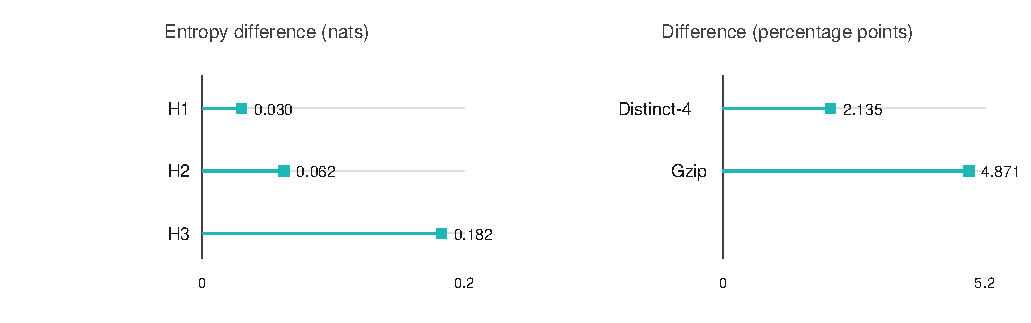
\includegraphics[width=0.9\textwidth]{figures/fig_diversity.pdf}
\caption{High-minus-Medium differences. Entropy differences are measured in
nats; $D_4$ and $\rho_{\rm gzip}$ differences are measured in percentage
points. Separate axes prevent heterogeneous quantities from sharing a common
bar scale.}
\label{fig:diversity}
\end{figure}

\begin{table}[ht]
\centering
\caption{Empirical risks of the historical checkpoints. Parameter counts
include vocabulary-dependent layers.}
\label{tab:results}
\begin{tabular}{llrrrr}
\toprule
Model & Corpus & Train & Test & Gap & Parameters\\
\midrule
Transformer & Medium & 1.7679 & 1.8355 & 0.0676 & 120,030\\
Transformer & High   & 1.9198 & 1.9597 & 0.0398 & 121,062\\
LLaMA-style & Medium & 1.3645 & 1.4638 & 0.0993 & 143,424\\
LLaMA-style & High   & 1.6268 & 1.7010 & 0.0742 & 144,448\\
\bottomrule
\end{tabular}
\end{table}

\begin{figure}[ht]
\centering
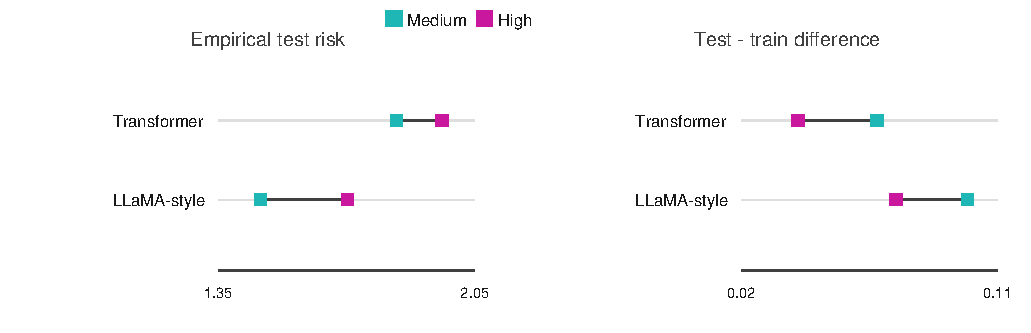
\includegraphics[width=0.9\textwidth]{figures/fig_results.pdf}
\caption{Test loss and the empirical test--train difference. Segments connect
corpora within an architecture; they are neither trajectories nor confidence
intervals. Perplexity is omitted because it is $\exp(\mathrm{loss})$ and has
exactly the same ordering.}
\label{fig:results}
\end{figure}

The High-minus-Medium test differences are $0.1241$ for the Transformer and
$0.2372$ for the LLaMA-style model. The corresponding gap differences are
$-0.0277$ and $-0.0251$. These signs describe the four stored checkpoints.
There are no independent repetitions from which to estimate variation across
initializations. Furthermore, High models have more parameters because
$K=102$ rather than $K=94$.

The new evaluator produces $L_{\rm uni}$, bpc, $G_{\rm ctx}$, and
$G_{\rm rel}$. They are not inserted into the historical table until all four
checkpoints have been evaluated under one versioned protocol. This restriction
prevents a report from silently combining artifacts generated under different
evaluation procedures.

\section{Logical scope and identifiability}

The observations establish only
\[
 \Delta_{\rm test}>0,
 \qquad
 \Delta_{\rm gap}<0
\]
for both architectures and for the stored realizations. They do not establish
that diversity increases expected risk or acts as an implicit regularizer. A
causal interpretation would require an intervention that changes diversity
while holding domain, alphabet, length, and semantic distribution fixed, as
well as independent training repetitions.

A smaller gap does not by itself order out-of-sample performance. A constant
predictor may have a zero gap and high risk. Here the smaller High gap coexists
with larger train and test losses. The phrase ``less overfitting'' can therefore
refer only to an empirical difference of losses, not to superior prediction.

An identifiable follow-up design should include:
\begin{enumerate}
 \item a family of corpora generated by an explicit random mechanism;
 \item an exactly shared character budget and a vocabulary fitted on train;
 \item matched parameter counts and target-position budgets;
 \item multiple seeds treated as independent experimental units;
 \item prespecified contrasts for raw loss, contextual gain, and interactions
       with architecture;
 \item blockwise evaluation or inference valid for dependent sequences.
\end{enumerate}
Varying data size and compute in addition would test whether diversity changes
the scaling rate, which is closer to the effective-token question than a
single-budget comparison.

\section{Conclusion}

The experiment separates three mathematical objects: descriptive diversity of
an observed string, predictive risk of a conditional model, and the empirical
test--train difference. In the stored runs, High has larger diversity
functionals, larger test loss, and a smaller gap. The evidence does not identify
a causal relation among these facts. The reproducible contribution is a formal
specification of the pipeline, an audit of its confounders, and an evaluation
scheme that compares absolute risk with contextual gain over a unigram
reference. The effective-token hypothesis remains open for a replicated and
controlled design.

\section*{Tool disclosure}
Language-model assistants were used for code review, manuscript restructuring,
and algebraic checks. Numerical statements are derived from versioned repository
artifacts. Responsibility for the content and conclusions remains with the
author.

{\small
\bibliographystyle{unsrtnat}
\bibliography{references}
}

\end{document}
